\documentclass[times,specification,annotation]{itmo-student-thesis}

%% Опции пакета:
%% - specification - если есть, генерируется задание, иначе не генерируется
%% - annotation - если есть, генерируется аннотация, иначе не генерируется
%% - times - делает все шрифтом Times New Roman, собирается с помощью xelatex
%% - languages={...} - устанавливает перечень используемых языков. По умолчанию это {english,russian}.
%%                     Последний из языков определяет текст основного документа.

%% Делает запятую в формулах более интеллектуальной, например:
%% $1,5x$ будет читаться как полтора икса, а не один запятая пять иксов.
%% Однако если написать $1, 5x$, то все будет как прежде.
\usepackage{icomma}

\newcommand{\Edelta}{$E[_{\Delta} X_t| X_t=I]$}
\newcommand{\EY}{$E[Y, X_t=I]$}
\newcommand{\EZdelta}{$E[_{\Delta} Z, X_t=I]$}
\newcommand{\P}{$P_{X_t = I}$}
\newcommand{\prn}{\frac{r}{n}}

%% Один из пакетов, позволяющий делать таблицы на всю ширину текста.
\usepackage{tabularx}

\usepackage{graphicx}
\graphicspath{{pictures/}}

%% Данные пакеты необязательны к использованию в бакалаврских/магистерских
%% Они нужны для иллюстративных целей
%% Начало
\usepackage{tikz}
\usetikzlibrary{arrows}


%% Указываем файл с библиографией.
\addbibresource{bachelor-thesis.bib}

\begin{document}

    \studygroup{M3437}
    \title{Теоретическое исследование эволюционного алгоритма (1+1) на динамических псевдобулевых задачах оптимизации}
    \author{Торопин Константин Игоревич}{Торопин К. И.}
    \supervisor{Максим Викторович Буздалов}{Буздалов М.В.}{к.т.н.}{}
    \publishyear{2021}
%% Дата выдачи задания. Можно не указывать, тогда надо будет заполнить от руки.
%%\startdate{01}{сентября}{2018}
%% Срок сдачи студентом работы. Можно не указывать, тогда надо будет заполнить от руки.
%%\finishdate{31}{мая}{2019}
%% Дата защиты. Можно не указывать, тогда надо будет заполнить от руки.
%%\defencedate{15}{июня}{2019}

    \secretary{Павлова О.Н.}

%% Задание
%%% Техническое задание и исходные данные к работе

%%% Содержание выпускной квалификационной работы (перечень подлежащих разработке вопросов)
    \plannedcontents{\begin{enumerate}
                         \item Постановка задачи
                         \item Описание
    \end{enumerate}}

%%% Исходные материалы и пособия

%%% Цель исследования
    \researchaim{Разработка теоретической базы для анализа эволюционных алгоритмов с динамически меняемыми функциями}

%%% Задачи, решаемые в ВКР
    \researchtargets{\begin{enumerate}
                         \item анализ возвращения алгоритма к оптимуму;
                         \item нахождение плато в зависимости от динамики;
                         \item проработка теории для анализа времени работы алгоритмов
                         \item проверка теории на практике
    \end{enumerate}}

%%% Использование современных пакетов компьютерных программ и технологий
    \addadvancedsoftware{Интегрированная среда разработки PyCharm}{\ref{sec:used_techs}}

%%% Краткая характеристика полученных результатов 
    \researchsummary{Расширена теоретическая база эволюционных алгоритмов на динамических псевдобулевых задачах оптимизации .}

%%% Гранты, полученные при выполнении работы 
    \researchfunding{Грантов и других форм государственной поддержки и субсидирования в процессе в процессе выполнения не предусматривалось.}

%%% Наличие публикаций и выступлений на конференциях по теме выпускной работы
    \researchpublications{Публикации и выступления, связанные с данной работой, отсутствуют.}

%% Эта команда генерирует титульный лист и аннотацию.
    \maketitle{Бакалавр}

%% Оглавление
    \tableofcontents

%% Макрос для введения. Совместим со старым стилевиком.

    \startprefacepage

    В практике применения эволюционных алгоритмов нередко встречаются динамические задачи оптимизации, в рамках которых функция выживания изменяется со временем.
    В теоретическом анализе времени работы эволюционных алгоритмов не так много работ уделяется этим задачам.
    И в этих работах центральным ставится вопрос может ли быть достигнут оптимум между изменениями функции приспособленности, а то, как в промежутке меняется значение приспособленности, не особо рассматривается, за вычетом приспособленностей, крайне близких к оптимуму.
    В частности не решается вопрос что должно происходить с различными способами адаптации параметров, которые применяются для повышения эффективности алгоритмов. Поэтому задача анализа алгоритма (1 + 1) на динамических псевдобулевых задачах оптимизации является актуальной.


    \chapter{Пояснительная записка}

    Эволюционные алгоритмы могут применяться для поиска экстремума функции.
    Однако в теории эволюционных алгоритмов существует проблема, которая заключается в том, что функция в процессе поиска экстремума может изменятся.
    Примером такой задачи может быть поиск оптимального маршрута в городе - искомый маршрут в зависимости от времени может отличаться.
    Поэтому возникает потребность проанализировать алгоритмы учитывая динамическое преобразование функции.
    Для начала был взят алгоритм (1 + 1) на задаче $OneMax$.

    Данный алгоритм был выбран потому что это наиболее понятная и простая задача для анализа и часто является отправной точкой для исследования.

    OneMax - задача поиска минимума функции количества несовпадающих бит с некоторым вектором $f_{max}$, длина которого $n$.

    Алгоритм (1 + 1) решает её следующим образом - берётся случайный вектор длины $n$ и далее итеративно мутируется - каждый бит независимо меняется с некоторой вероятностью $\frac{r}{n}$ ($r$ рассматривается в данном исследовании $o(1)$ по отношению к $n$).
    Если количество совпадающих бит увеличивается, берётся мутируемый.
    Добавим следующую динамику для задачи - пусть каждые $T$ итераций алгоритма вектор $f_{max}$ меняет один случайный бит.

    В рамках исследования были выявлены две ситуации - когда $T$ слишком мала, то алгоритм "застревает"  на некотором значении, расстояние до $f_{max}$ колеблются на уровне некоторого $с \cdot n$.
    Значение $c$ будем называть точкой стабилизации или плато.
    То есть в этой ситуации с некоторого момента примерное отношение бит которые не совпадают с вектором $f_{max}$ ко всем битам будет равна $c$.
    Вторая ситуация - $T$ оказывается достаточно большой, что алгоритм доходит до нужного оптимума, однако медленнее чем если бы динамики не было.
    Помимо этого был рассмотрена ситуация когда алгоритм не заканчивается на достижении оптимума (что вполне можно увидеть на реальных задачах).
    Тогда будет разумным вопрос - какая вероятность, что при изменении одного бита алгоритм успеет найти новый оптимум до следующего изменения.

    По первому случаю был установлен факт, что значение $c$ не зависит от параметра $T$ (если $n > 1/c$), это значит что если мы фиксируем какое-то значение $T$, то насколько сильно мы бы не увеличивали $n$, значение $c$ будет оставаться тем же.
    Были найдены некоторые оценки на значение $c$, а так же теоретически обоснован факт почему алгоритм фиксируется и почти не уходит от этого значения.

    Что касается второго случая - асимптотика EA-алгоритмов обычно оценивается с помощью некоторых теорем которые несут общее название drift-analysis.
    Были взяты теоремы Additive Drift и Variable Drift и рассмотрены с точки зрения того, что математическое ожидание изменения функции на некоторых шагах отличается от обычного.
    Если рассматривать данную конкретную задачу, то в ней каждые $K$ шагов математическое ожидание будет отличаться на некоторое значение $\leq 1$.
    Эти теоремы в дальнейшим могут помочь исследовать скорость нахождения первого оптимума и в более сложных алгоритмах в которых будет введена динамика.
    С помощью видоизмененных теорем была доказано, что если $T$ больше некоторого значения, то асимптотика алгоритма не изменится, то есть останется $O(n \cdot log(n))$

    По последнему вопросу были рассмотрены ситуации в которых вероятность нахождения нового оптимума быстрее чем придёт новое изменение равна $o(1)$ и $1 - o(1)$.
    Так же и найдены границы для $T$ чтобы вероятность была больше или меньше заданного значения.

    Экспериментальные данные показывают, что плато находится на тех значениях, которые предсказывает теория.

    \chapter{Теоретическое исследование}

    \section{Постановка задачи}
    TODO - пояснение что такое OneMax, LeadingOnes (1 + 1) и как вводится динамика + псеводокоды. Ввести величины $p = \frac{r}{n}$ и $q = 1 - p$ - вероятность изменения одного бита.

    Исследование задачи эволюционных алгоритмов с динамическими изменениями достаточно плохо изучены.
    Существует исследования на эту тему [ссылка] в которых основной упор делается на скорость работы алгоритма, но не на анализ его поведения.
    Так же в этих исследованиях не используется Drift анализ [ссылка], часто используемый для анализа скорости работы,
    поэтому было принято решение сформулировать некоторые известные теоремы с учётом динамических изменений, чтобы можно было из использовать в анализе более сложных алгоритмов.

    В ходе практического анализа алгоритма была обнаружена закономерность, что алгоритм при некоторых значениях параметра $T$ алгоритм "останавливается" в некоторых точках.

    Для дальнейшего анализа нам потребуются обозначения:
    Todo описать что такое X - количество бит совпадающие с вектором, Y - процесс увеличения и Z - процесс уменьшения, формально написать что значат эти величины и что мы внутри скрываем фильтрацию сигма алгебр.
    Сейчас для понимания: есть величина случайная величина $X_t$ - количество бит на шаге t, $Y_t$ - её "прирост на шаге t" за счёт алгоритма, $Z_t$ - его уменьшение.
    То есть $X_t = \sum_{0}^{t - 1} Y_t - Z_t $
    \section{Поиск плато}

    В ходе практического исследования алгоритма был установлен факт, что для некоторых T значение алгоритм останавливается на некотором значении и не может далеко уйти за эти рамки.
    Назовём значение этой точки "плато" и будем искать его в следующей точке: пусть I - количество совпадающий бит, n - длинна массива где математическое ожидание "подняться вверх" то есть на сколько больше бит будет будет равняться оптимальному будет равно значению \frac{I}{T \cdot n}.
    Физический смысл этого можно понять так: пусть мы рассматриваем задачу, когда динамика может происходить каждый раз, но с вероятностью 1/T.
    Вероятность того, что динамика ухудшит ответ будет \frac{I}{T \cdot n} и математическое ожидание будет процесса динамики будет равно этому же \frac{I}{T \cdot n}.
    Так что суммарное математическое ожидание будет равно 0.
    На самом деле задача стоит другим образом и честная оценка E[X_{t+T} - X_t, x_t = I] через T итераций будет ниже чем T \cdot E[\deltaX, x_t = I] потому что она убывает от роста I, но заглядывая в будущее, окажется что этого приближния достаточно, и уйти от данной точки на линейную длину алгоритму будет экспонециально сложно.

    Пусть в данный момент у алгоритма величина $X_t = I$, то есть количество бит текущего, которые совпадают с текущим оптимальным вектором.
    Введём обозначения - для конкретной $I$
    \begin{gather*}
        Bin(m, n) \equiv C_m^n \cdot p^{m} \cdot q^{n - m} = C_m^n \cdot p^{m} \cdot q^{n - m}\\
        A(i) \equiv Bin(i, I)\\
        Q(i) \equiv Bin(i, n - I)\\
        с = \frac{I}{n}\\
    \end{gather*}
    Значение $c$ можно рассматривать как процент правильных бит.
    Значение $A(i)$ как вероятность что среди $I$ бит произойдёт ровно $i$ изменений.
    Значение $Q(i)$ как вероятность что среди $n - I$ бит произойдёт ровно $i$ изменений.

    Так как вероятность изменения значения вектора ровно на $i$ равна вероятности того что среди ещё не найденных бит изменится ровно $k$ бит, а в найденных изменится $k - i$ для всех возможных $k$.

    \begin{gather*}
        P(Y_t = i|X_t=I) = \sum_{j=1}^{\min(I - i, n - I - i)} A(i + j)Q(i)
    \end{gather*}

    Давайте рассматривать только такие $I$ что
    \begin{gather*}
        c > 0.5 \\
        c \cdot r < 1 \\
    \end{gather*}
    Вероятностный смысл будет высказан позже.
    Заметим что
    \begin{gather*}
        P(Y_t = i|X_t=I) = \sum_{j=1}^{I - i} A(i + j)Q(i)
    \end{gather*}
    Тогда значение \EY можно расписать в виде:
    $\EY = \sum_{i=1}^I i \cdot \sum_{j=1}^{I - i} A(i + j)Q(i) = \sum_{i=1}^I Q(i) \sum_{j=i}^{I} j \cdot A(j - i)$
    \begin{align*}
        Q(0)A(1) + && 2\cdotQ(0)A(2) && + 3\cdotQ(0)A(3) && + {}\ldots{} && + I\cdotQ(0)A(I) + & \\
        && Q(1)A(2)   && + 2\cdotQ(1)A(3) && + {}\ldots{} && + (I-1)\cdotQ(1)A(I)  + &\\
        && && && + {}\ldots{} && + \vdotswithin{A(I)Q(n - I)} + & \\
        && && && && + A(I)Q(n - I) + &
    \end{align*}

    Так как $\sum_{j=1}^{I} j \cdot A(j)$ это определение матожидание случайной величины $A$, что равно $pI$
    Заметим что первая строчка равна
    $\tau^* \equiv Q(0) \cdot \sum_{j=1}^{I} j \cdot A(j) = Q(0) \cdot pI = q^{n - I} \cdot c \cdot r$
    Это будет нашей нижней оценкой на \EY
    Далее оценим сумму остальных строчек.
    Давайте оценим сверху для каждой строчки во сколько изменяется элемент в строчке относительно предыдущего:
    Для строчки $i$:
    $i \geq 2 \n i \geq 1$
    \begin{gather*}
        \frac{(j + 1)\cdot Q(i)\cdot A(i + j + 1)}{j\cdot Q(i) \cdot A(i + j)} \\
        = \frac{j + 1}{j} \cdot \frac{(I - (i + j + 1))!}{I! \cdot (i + j + 1)!} \cdot p^{I - (i + j + 1)} q^{i + j + 1} \frac{I! \cdot (i + j)!} {(I - (i + j))!} \cdot \frac{1}{p^{I - (i + j)} q^{i + j}} \\
        = \frac{j + 1}{j} \cdot \frac{I - i - j}{i + j + 1} \cdot (\frac{q}{p} = \frac{r \cdot n}{n \cdot (n - r)} = \frac{r}{n - r}) \\
        =  \frac{j + 1}{j \cdot (i + j + 1)} \cdot  \frac{c\cdot(n - r) + c\cdotr - i - j - 1}{n - r} \cdot r \leq \\
        \leq \frac{1}{2} \cdot \frac{c\cdot(n - r)}{n - r} \cdot r = \frac{c \cdot r}{2}
    \end{gather*}
    Значит каждая строчка $i$:
    \begin{gather*}
        a_i \equiv \sum_{j = 1}^{i - i} (j \cdot Q(i) \cdot A(i + j)) = \\
        = \sum_{j = 1}^{inf} (Q(i) \cdot A(i + 1) \cdot (\frac{c \cdot r}{2})^{0}) \\
        = Q(i) \cdot A(i + 1) \cdot \frac{1}{1 - \frac{c \cdot r}{2}}
    \end{gather*}

    Аналогично проделаем с данным рядом:
    \begin{gather*}
        \frac{Q(i + 1) \cdot A(i + 2)}{Q(i) \cdot A(i + 1)} = \frac{(n - I - i) \cdot (I - i - 1)}{(i + 1) \cdot (i)} \cdot (\frac{r}{n - r})^2 \\
        = \frac{(n - r)\cdot(1 - c) + r - r\cdotc - i}{n - r} \cdot \frac{c\cdotn - r\cdotc - r\cdotc - i - 1}{n - r} \cdot \frac{1}{(i + 1) \cdot (i)} \\
        \leq (1 - c) \cdot c \cdot 1/2 + (\frac{(r - r\cdotc - i) \cdot c \cdot 1/2}{n - r} = \theta(1))
    \end{gather*}
    C другой стороны, если брать $n >= r/c$
    \begin{gather*}
        c \cdot 1/2 \cdot \frac{n - nc - I}{n - r} \leq \\ c \cdot 1/2 \cdot \frac{n - r - I}{n - r} < c \cdot 1/2
    \end{gather*}

    Давайте рассмотрим оценку $c/2$, тогда получается, что вся остаточная часть меньше или равна по аналогии:

    \begin{gather*}
        Q(1)A(2) \cdot \frac{1}{1 - c/2} \cdot \frac{1}{1 - c \cdot r/2} = \frac{(n - I)\cdotI\cdot(I - 1)}{2} \cdot p^3 \cdot q^{n - 3} \cdot constants \leq\\
        \leq c^2 \cdot r^3 \cdot q^{n - 3} = (q^{n - I} \cdot c \cdot r) \cdot  (q^{I + 3} \cdot c \cdot r^2)  = \tau^* \cdot (q^{I + 3} \cdot c \cdot r^2)
    \end{gather*}
    Значение $constants < 1$ его можно использовать, чтобы брать более качественные оценки на $c_{lower}$ о котором будет говорится позже. \\

    Оценки $\tau^*$:

    Введем значение $\tau \equiv \exp(-r + r\cdotc) \cdot c \cdot r$ \\
    \begin{gather*}
        \tau^* = q^{n - I} \cdot c \cdot r = (1 - r/n)^n \cdot (1 - c) \cdot c \cdot r < \exp(-r + r\cdotc) \cdot c \cdot r = \tau\\
        \tau^* = (1 - r/n)^{n - r}\cdot(1 - c) \cdot c \cdot r \cdot (1 - r/n)^{r}\cdot(1 - c) \\
        > \exp(-r + r\cdotc) \cdot c \cdot r \cdot (1 - r^2/2n)^{1 - c} > \\
        \exp(-r + r\cdotc) \cdot c \cdot r \cdot (1 - r^2/2n) > \exp(-r + r\cdotc) \cdot c \cdot r \cdot (1 - o(1)) = \tau \cdot (1 - o(1))\\
    \end{gather*}
    Заметим так же:
    \begin{gather*}
        q^{I + 3} = (1 - r/n)^{c + 3} <~\eqref{exp:less}< \exp(-r \cdot c) \cdot (1 - r/n)^3 < \exp(-r\cdotc)\\
    \end{gather*}
    Обозначим $k \equiv \exp(-r\cdotc) \cdot c \cdot r^2$ \\
    Тогда сумма всей таблицы оценивается сверху как: \\
    \begin{gather*}
        \tau^* \cdot (1 + q^{I + 3} \cdot c \cdot r^2)  < \exp(-r + r\cdotc) \cdot c \cdot r \cdot (1 + \exp(-r\cdotc) \cdot c \cdot r^2) < \tau \cdot (1 + k)
    \end{gather*}

    Из чего сделаем вывод что $\EY  \in (\tau \cdot (1 - o(1)), \tau \cdot (1 + k))$ \\

    Рассмотрим \EZdelta. \\
    Для начала давайте рассматривать задачу в которой каждый шаг с вероятностью $1/T$ меняется один бит в векторе $f_{\max}$\\
    Связь с истинной задачей будет рассматриваться позже.
    Так как вероятность что случайно выбранный бит будет из тех, которые уже достигли оптимума равняется $1 - I/n = (1 - c)$
    Тогда
    \[
        \EZdelta = (1 - c)/T
    \]
    Заметим что $\EZdelta$ возрастает с убыванием $c$, когда как \EY убывает.\\
    Второй факт доказывается тем что при $p > 1/2$ вероятность изменить бит > $\frac{1}{2}$, а количество необходимых бит убывает. (Можно доказать строже)
    Тогда рассмотрим для фиксированного $T$ такие два значения $c_{upper}$ и $c_{lower}$ для которых мы можем быть уверены что:

    \begin{gather*}
        E[_{\Delta}(X_t)| X_t = n \cdot c_{upper}] > 0
        E[_{\Delta}(X_t)| X_t = n \cdot c_{lower}] < 0
    \end{gather*}

    Грубо говоря вне этого промежутка алгоритм будет "тянуть" его назад.

    \begin{gather*}
        E[_{\Delta}(X_t)| X_t = n \cdot c] = \E[_{\delta}(Y_t)| X_t = n \cdot c] - \frac{(1 - c}{K} \\
        \EY \in (\tau - o(1), \tau \cdot (1 + k)) \\
        0 \leq \E[_{\Delta}(X_t)| X_t = n \cdot c] < \tau - o(1) - \frac{(1 - c}{K} \\
        K \cdot (\tau - o(1)) > (1 - c) \\
        K > \frac{(1 - c)}{\tau \cdot (1 - o(1))} \\
    \end{gather*}

    Рассмотрим $g_{lower}(c) = \frac{(1 - c)}{\tau} = \frac{(1 - c)}{\exp(-r + r\cdotc) \cdot c \cdot r}$ \\

    Тогда $c_{lower} = g_{lower}^{-1}(K) + \epsilon$ где $\epsilon \rightarrow 0$ для больших $n$ (TODO формальнее) \\

    Аналогично $g_{upper}(c) = \frac{(1 - c)}{\tau \cdot (1 + k)} =  \frac{(1 - c)}{\exp(-r + r\cdotc) \cdot c \cdot r \cdot (1 + \exp(-r\cdotc) \cdot c \cdot r^2)}$\\
    $c_{upper} = g_{upper}^{-1}(K)$ \\

    Заметим что величины $c_{upper}$ и $c_{lower}$ не зависят от $n$, а значит мы можем сделать вывод что плато будет начинаться в одинаковых значениях вне зависимости от величины $n$.

    Далее оценим величину:
    \begin{gather*}
        P(_{\Delta} Y \geq j|Y_t = I)
    \end{gather*}

    Установим следующий факт:

    \begin{theorem}
        \begin{gather*}
            \exist r, \eta > 0, I > n/2: \\
            P(_{\Delta} Y \geq j|Y_t = I) \leq \frac{r}{(1 + \eta)^j}
        \end{gather*}
    \end{theorem}

    \begin{proof}
        \begin{gather*}
            P(j) \eq P(_{\Delta} Y = j|Y_t = I) = \sum_{i = 0}^{I - j} A(i + j)Q(i) \\
            \frac{A(i)}{A(i + 1)} = \frac{n!}{i! \cdot (n - i)!} \cdot p^i \cdot q^{n - i} \cdot \frac{(i + 1)! \cdot (n - i - 1)!}{n!} \cdot \frac{1}{p^{i + 1} \cdot q^{n - i - 1}} = \\
            = \frac{i + 1}{n - i} \cdot \frac{n - r}{r}
            P(_{\Delta} Y \geq j|Y_t = I)
        \end{gather*}

    \end{proof}


    Тогда используя Negative-drift теорему мы можем доказать что уйти на любое значение от плато займёт экспоненциальное время.

    \begin{theorem}
        Пусть $X_{t_0} = c: c \in (c_{lower}, c_{upper})$
        Тогда найдётся такое большое $n$, что:
        \begin{gather*}
            1. \forall k : k > 1/2, k \cdot n < c_{lower} \cdot n - 1, \\
            T_a = \min{t > t_0 | X_t \leq k \cdot n} \exists l: \\
            P[T_a \leq e^{l\cdotn}] < e^{-l\cdotn} \\
            2. \forall k : k  \leq 1, k \cdot n > c_{upper} \cdot n + 1, \\
            T_a = \min{t > t_0 | X_t \geq k \cdot n} \exists l: \\
            P[T_a \leq e^{l\cdotn}] < e^{-l\cdotn} \\
        \end{gather*}
    \end{theorem}

    \begin{proof}
        Из факта выше следует, что для всех $I > 1/2$ \\
        $P(_{\Delta} Y \geq j|Y_t = I) \leq \frac{r}{(1 + \eta)}$ \\
        Так же заметим что $Z_t$ не может превышать по модулю 1 \\
        \begin{gather*}
            P(_{\Delta} Z \geq 1) \leq \frac{1}{K}
            P(_{\Delta} Z \geq j > 1)= 0
        \end{gather*}
        Таким образом: \\
        $P(|_{\Delta} X| \geq j|X_t = I) \leq \frac{\max(r, 1/K)}{(1 + \eta)}$ \\

        1. Рассмотрим второй случай, так как \Edelta убывает и $E[_{\Delta} X| X_t = c_{upper} \cdot n] \equiv \delta < 0$ \\
        И по монотонности для всех
        \begin{gather*}
            I \in (c_{upper} \cdot n, k \cdot n)
            E[_{\Delta} X| X_t = I] < \delta < 0
        \end{gather*}
        Таким образом все условия Negative-Drift теоремы выполнены. \\

        2. Аналогично, только рассмотрим вместо $X_t$ случайную величину $W_t = -X_t$, тогда \\
        \begin{gather*}
            E[_{\Delta} W| W_t = c_{lower} \cdot n] \equiv \delta < 0 \\
            I \in (k \cdot n, c_{lower} \cdot n)  \\
            E[_{\Delta} W| W_t = I] \equiv \delta < 0 \\
        \end{gather*}
    \end{proof}

    TODO: показать какие конкретно $l$ и $n_0$ и что вообще с этим можно делать - построение честного вероятностного удалось сделать с помощью марковский цепей.\\
    Однако только снизу и если брать более слабую теорию где не $EY > EZ$, а $PY > PZ$, что мало чего даёт. \\
    Наверное всё же нужно просто доказать что мы постоянно будем возвращаться в это плато, но хотелось бы чего-то лучше.


    \section{Оценки скорости нахождения первого оптимума}
    Рассмотрим классические Drift-теоремы с точки зрения задачи.
    \begin{theorem}
        \label{drift:add}
        Пусть $(X_t)_{t \in N}$, последовательность случайных величин с $S \in [0, \infty)$ состояниями\\
        $X$ \in $Z$ \\
        $s_{\min} = \inf(S \backslash \{0\})$ \\
        Пусть $T := \inf{t > 0 | X_t = 0}$. \\
        Для любого $t \geq 0 : \\
        \delta_t(s) = E[X_t - X_{t + 1}| t \% K \neq K - 1, X_t = s]\\
        \Delta_t(s) = E[X_t - X_{t + 1}| t \% K = K - 1, X_t = s]$\\
        Если существуют такие константы $\epsilon$ и $\delta$, что:\\
        \begin{gather*}
            \epsilon \cdot K > \delta \\
            \delta_t(s) > \epsilon \\
            \Delta_t(s) > \epsilon - \delta
        \end{gather*}
        Тогда $E[T] \leq \frac{E[X_0]}{\delta - \epsilon/K}$  \\
    \end{theorem}
    \begin{proof}
        Теорему можно свести к классической теореме об Аддитивном дрифте. %ссылка
        Рассмотрим случайную величину $Y_i = X_{i \cdot K}$
        \begin{gather*}
            E[Y_0] = E[X_0] \\
            Y_{i + 1} = X_i \cdot k + \sum_{t=i \cdot K}^{i \cdot (K + 1) - 1} (X_{t + 1} - X_{t}) + \delta \\
            E[Y_i - Y_{i + 1}] \geq  K \cdot \epsilon - \delta > 0 \\
        \end{gather*}
        Последнее неравенство из условия. \\
        Тогда если $I$ - первое такое $i$, что $Y_i = 0$, $E[I] \leq \frac{E[X_0]}{K \cdot \epsilon - \delta}$. \\
        А значит $E[T] \leq E[I] \cdot K \leq \frac{E[X_0]}{\epsilon - \frac{\delta}{K}}$
    \end{proof}

    Теперь рассмотрим вариативный дрифт:

    \begin{theorem}
        \label{drift:var}
        Пусть $(X_t)_{t \in N}$, последовательность с $S \in [0, \infty)$ состояниями, число $K$
        $s_{\min} = \inf(S \backslash \{0\})$
        Пусть $T := \inf{t > 0 | X_t = 0}$.
        И для любого $t \geq 0 : \\
        \delta_t(s) = E[X_t - X_{t + 1}| t \% K \neq K - 1, X_t = s] \\
        \Delta_t(s) = E[X_t - X_{t + 1}| t \% K = K - 1, X_t = s]$ \\
        Если существуют такая константа $\epsilon$ и монотонно возрастающая функция $h : R^+ \rightarrow R^+$ что:
        \begin{gather*}
            \delta_t(s) > h(s) \\
            \Delta_t(s) > h(s) - \epsilon \\
            K > \frac{\epsilon}{h(s_{\min})}
        \end{gather*}
        Тогда:
        \begin{gather*}
            E[T] \leq \frac{1}{{1 - \frac{\epsilon}{K \cdot h(s_{\min})}}}  \cdot
            (\frac{s_{\min}}{h(s_{\min})} + E[\int_{s_{\min}}^{X_0}\frac{1}{h(\sigma)}d\sigma])
        \end{gather*}
    \end{theorem}
    \begin{proof}
        Воспользуемся доказательством классического вариативного дрифта.\\ %ссылка
        Если рассматривать функцию
        g(s) := \begin{cases}
                    \frac{s_{\min}}{h(s_{\min})} + \int_{s_{\min}}^{s}\frac{1}{h(\sigma)}d\sigma, &\mbox{if } s \geq s_{\min} \\
                    \frac{s_{\min}}{h(s_{\min})}, &\mbox{if } 0 \leq s \leq s_{\min}
        \end{cases}
        То по некоторым свойствам (здесь можно подробно расписать, но это уже есть в самой теореме) получается что если брать $Y_t = g(X_t)$: \\
        Для $t \mod K \neq K - 1$ : \\
        \begin{gather*}
            E[Y_t - Y_{t + 1}|Y_t = g(s)] = E[g(X_t) - g(X_{t + 1})| g(X_t) = g(s)] \\
            \geq E[\frac{X_t - X_{t + 1}}{h(X_t)}] = \frac{\delta_t(s)}{h(s)} \geq 1
        \end{gather*}
        Для $t \mod K = K - 1$: \\
        \begin{gather*}
            E[Y_t - Y_{t + 1}|Y_t = g(s)] \geq \frac{\Delta_t(s)}{h(s)} \geq 1 - \frac{\epsilon}{h(s_{\min})}
        \end{gather*} \\

        Тогда можем применяя~\eqref{drift:add} выше со следующими условиями: \\
        \begin{gather*}
            \epsilon_{new} \equiv 1 \\
            \delta_{new} \equiv \frac{\epsilon}{h(s_{\min})} \\
            K_{new} \equiv K \\
            K > \frac{\epsilon}{h(s_{\min})} > \delta_{new} \\
            \epsilon_{new} \cdot K_{new} > \delta_{new}
        \end{gather*} \\
        Значит: \\
        \begin{gather*}
            E[T] \leq \frac{1}{1 - \frac{\epsilon}{K \cdot h(s_{\min})}} \cdot (\frac{s_{\min}}{h(s_{\min})} + E[\int_{s_{\min}}^{X_0}\frac{1}{h(\sigma)}d\sigma])
        \end{gather*}
    \end{proof}


    Применим данную теорему к рассматриваемой задаче: \\

    \begin{theorem}
        Если Алгоритм $OneMax(K)$ имеет
        $K = O(n)$, $K > \frac{n \cdot \exp(r)}{r} + O(n)$, то
        $E[T] = O(n \cdot \log(n))$
    \end{theorem}
    \begin{proof}
        \begin{gather*}
            \delta_t(s) \geq A(1)Q(0) = i \cdot p \cdot q^{n - 1} = i \cdot r/n \cdot (1 - r/n)^{n - 1} \\
            \geq \frac{i}{n} \cdot r \cdot \exp(-r) - \phi(n) \\
            \phi(n) = o(1/n) \\
            \Delta_t(s) = \delta_t(s) - \frac{n - s}{n} \geq \delta_t(s) - 1 \\
            \epsilon = 1\\
            s_{min} = 1 \\
            h(s) = r \cdot \frac{s}{n} \cdot \exp(-r) - \phi(n) \\
            h(s_{min}) = \frac{r \cdot \exp(-r)}{n} - \phi(n) \\
            K > \frac{1}{h(s_{\min})} \\
            \exists c \in (0, 1): \frac{1}{1 - \frac{1}{K \cdot h(s_{\min})}} < c \\
        \end{gather*}
        Значит мы можем применить теорему~\eqref{drift:var}:
        \begin{gather*}
            E[T] \leq \frac{1}{1 - \frac{\epsilon}{K \cdot h(s_{\min})}} \cdot (\frac{s_{\min}}{h(s_{\min})} + E[\int_{s_{\min}}^{X_0}\frac{1}{h(\sigma)}d\sigma]) = \\
            = c \cdot (O(n \cdot \log(n))) = O(n \cdot \log(n))
        \end{gather*}

    \end{proof}


    \section{Добавочные леммы}

    Леммы про свойства экспоненты:
    \begin{lemma}
        \label{exp:less}
        $(1 - r/n)^n < e^{-r}$
    \end{lemma}

    \begin{lemma}
        \label{exp:greater}
        $(1 - r/n)^{n - r} > e^{-r}$
    \end{lemma}

    \begin{lemma}
        \label{exp:greater2}
        $(1 - r/n)^r > 1 - 2r/n$
    \end{lemma}
    \begin{proof}
        Пусть $a$ - такое что $a = 2^k, a \leq r, 2\cdota > r$, где $k \in \mathbb {N}$ \\
        \begin{gather*}
            (1 - r/n)^r \geq (1 - r/n)^a = (1 - 2r/n + r^2/n^2)^{a/2} > (1 - 2r/n)^{a/2} \\
            > (1 - 4r/n)^{a/4} > 1 - a\cdotr/n > 1 - 2\cdotr^2/n
        \end{gather*}
    \end{proof}

    \begin{lemma}
        \label{exp:greaterO}
        $(1 - r/n)^n > e^{-r} \cdot (1 - o(1/n))$
    \end{lemma}
    \begin{proof}
        \begin{gather*}
            (1 - r/n)^n > e^{-r} \cdot (1 - r/n)^r > e^{-r} \cdot (1 - 2 \cdot r^2/n) > e^{-r} - o(r^2/n) = e^{-r} - o(1)
        \end{gather*}
    \end{proof}


    \chapter{Проверка гиппотез на реальных данных}\label{ch:проверка-гиппотез-на-реальных-данных}

    Для того чтобы посмотреть насколько быстро будет возвращаться алгоритм после первого достижения оптимума были проведён следующий эксперимент: \\
    Алгоритм запускается несколько раз на одних и тех же $n$ и $T$.
    И рассматривается количество раз, когда алгоритм успевает найти новый оптимум. \\
    $\mu$ - матожидание первого срабатывания. \\
    \begin{figure}[H]
        \centering
        \caption{Как часто алгоритм найти успевает новый оптимум при n = 20}
        \label{pic:sublists-metafile}
        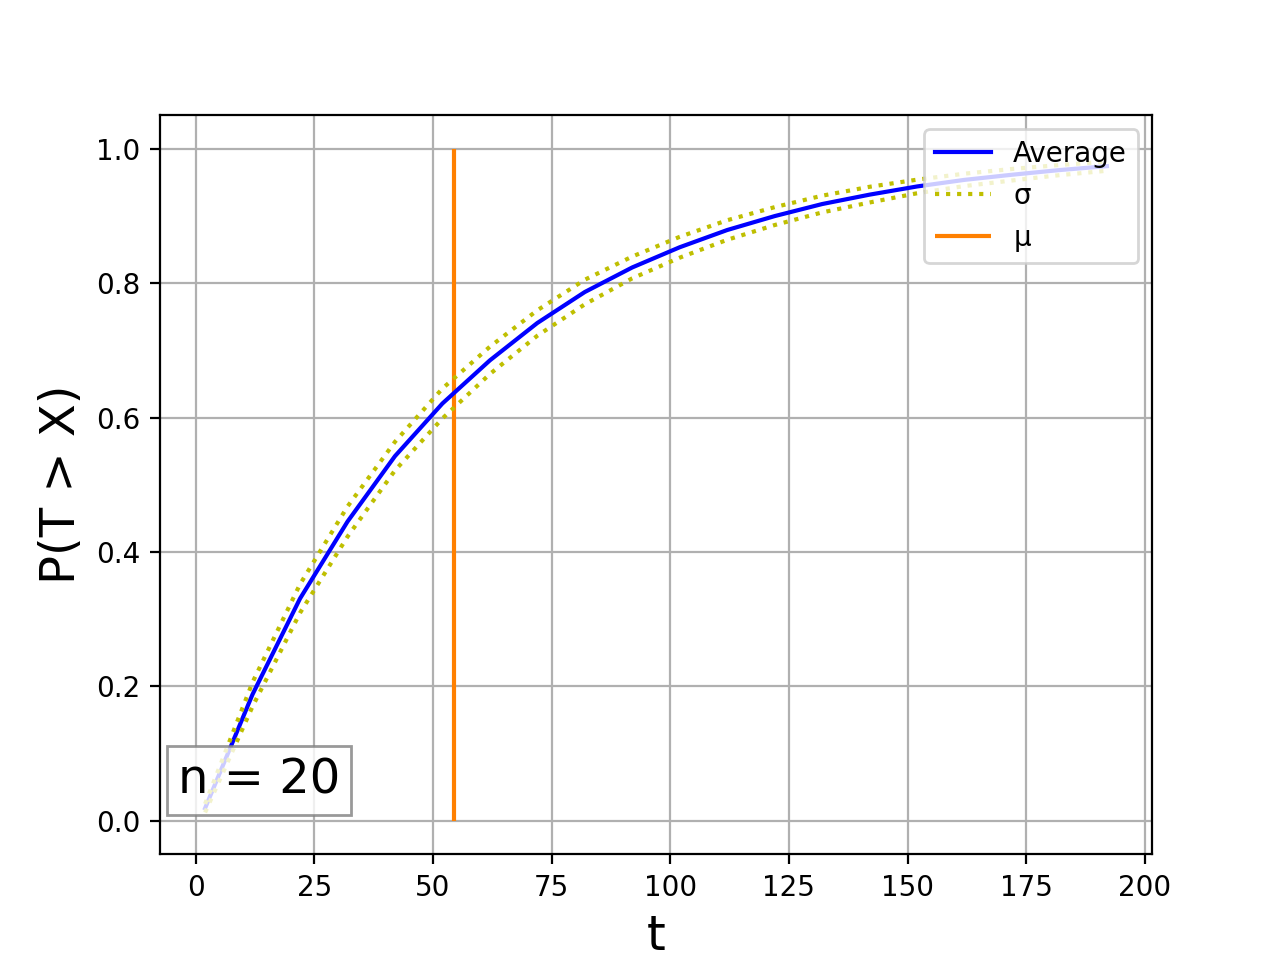
\includegraphics[scale=0.8]{plot_T_bigger_X_20.png}
    \end{figure}

    \begin{figure}[H]
        \centering
        \caption{Как часто алгоритм найти успевает новый оптимум при n = 40}
        \label{pic:sublists-metafile}
        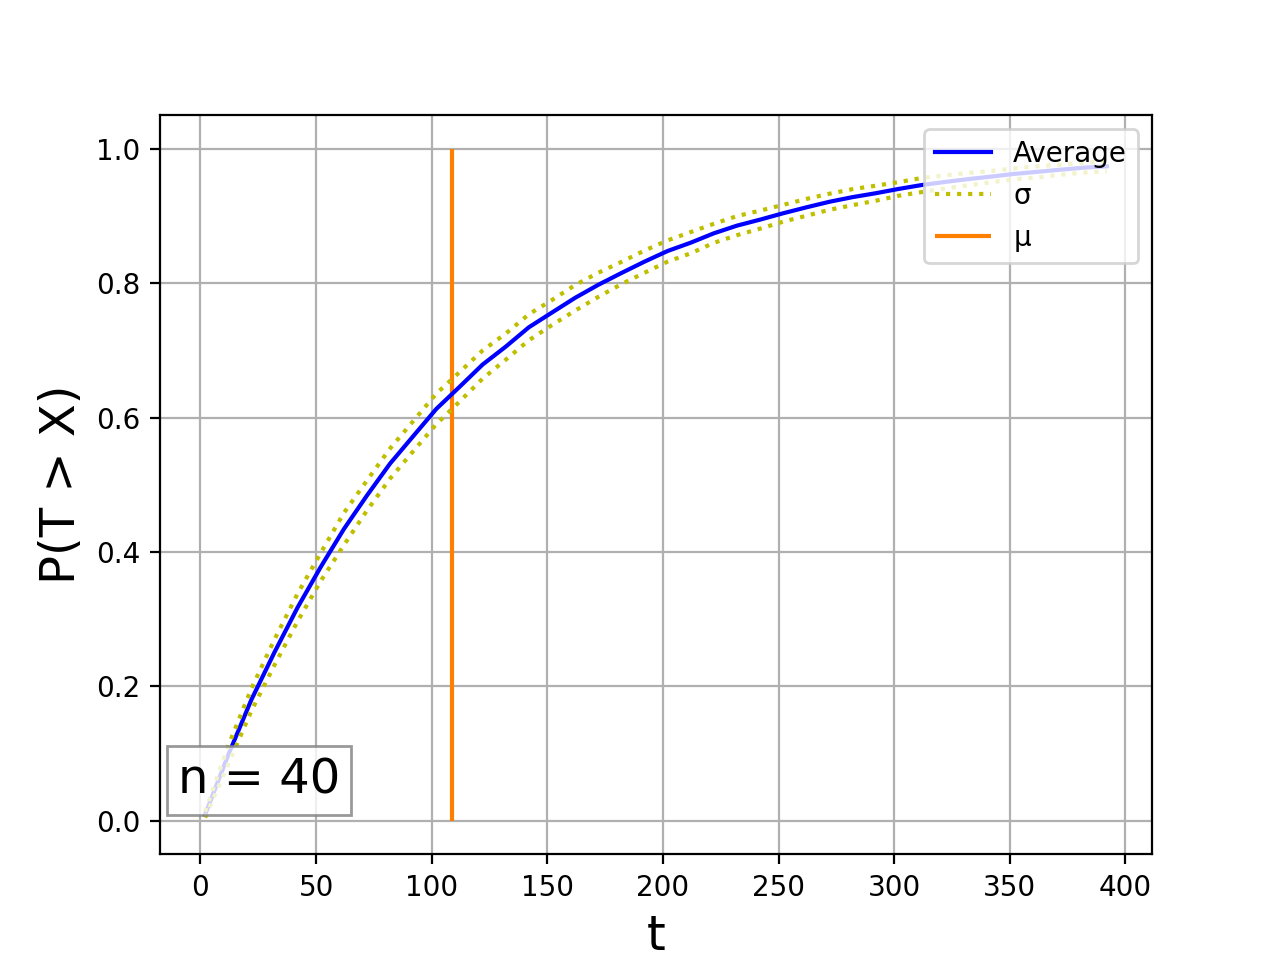
\includegraphics[scale=0.8]{plot_T_bigger_X_40.png}
    \end{figure}

    Для оценки скорости алгоритма так же рассматриваются разные значения $T$
    \begin{figure}[H]
        \centering
        \caption{Время работы алгоритма с n = 30}
        \label{pic:sublists-metafile}
        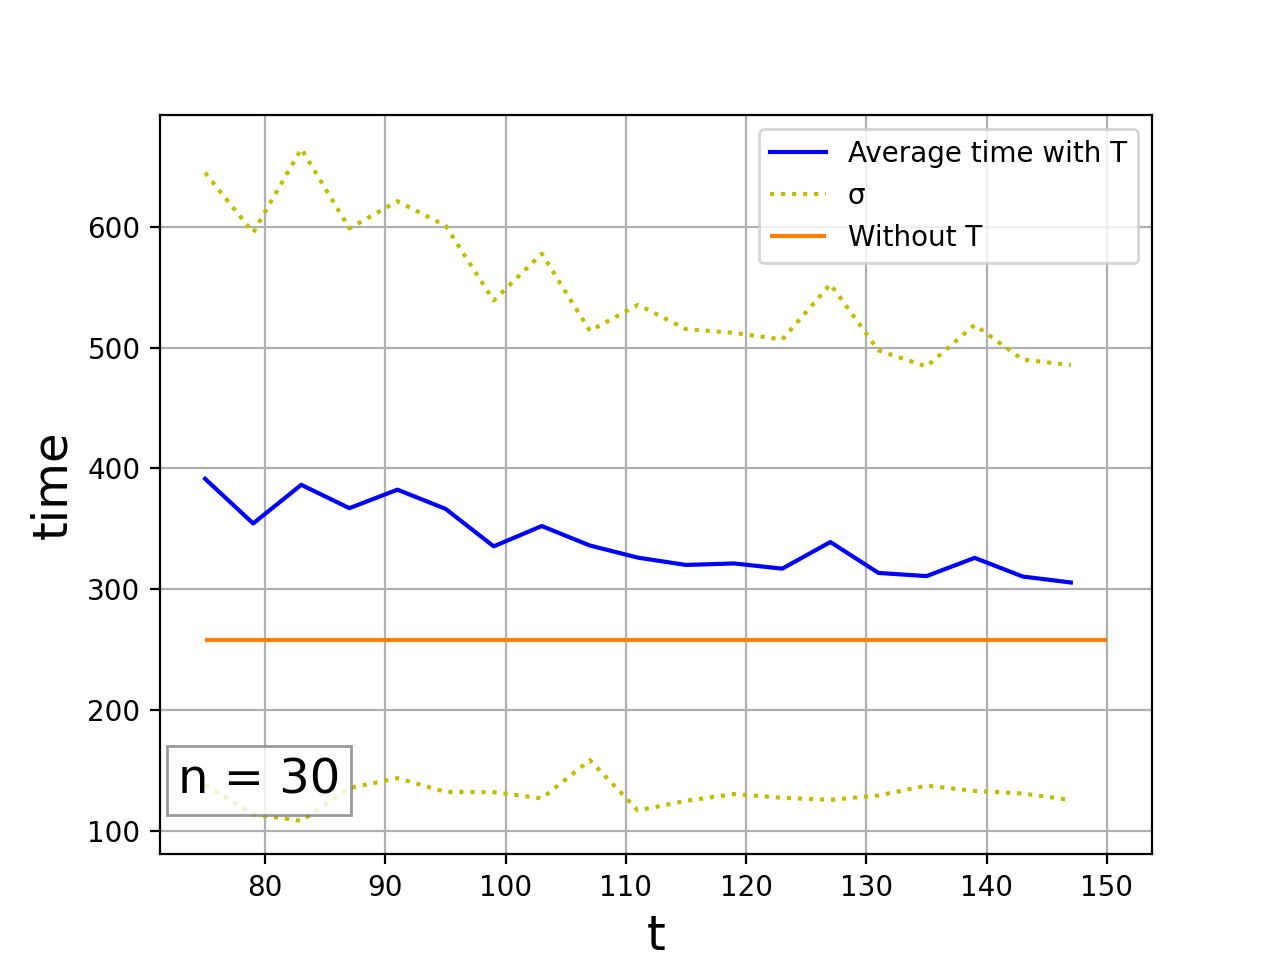
\includegraphics[scale=0.8]{plot_time_30_as_30.png}
    \end{figure}


    В качестве демонстрации основной гипотезы о независимости значения плато от $n$ поставлены несколько экспериментов с разными $n$, но с одной и той же $T = 20$. \\
    На графиках изображено усредненное поведение функции $d$ - количество разных бит у $f$ и $f_{\max}$ за 20 запусков. \\
    Как видно из экспериментов они все останавливаются примерно на одном уровне по отношению к $n$. \\
    \begin{figure}[H]
        \centering
        \caption{Обнаружение плато с n = 100}
        \label{pic:sublists-metafile}
        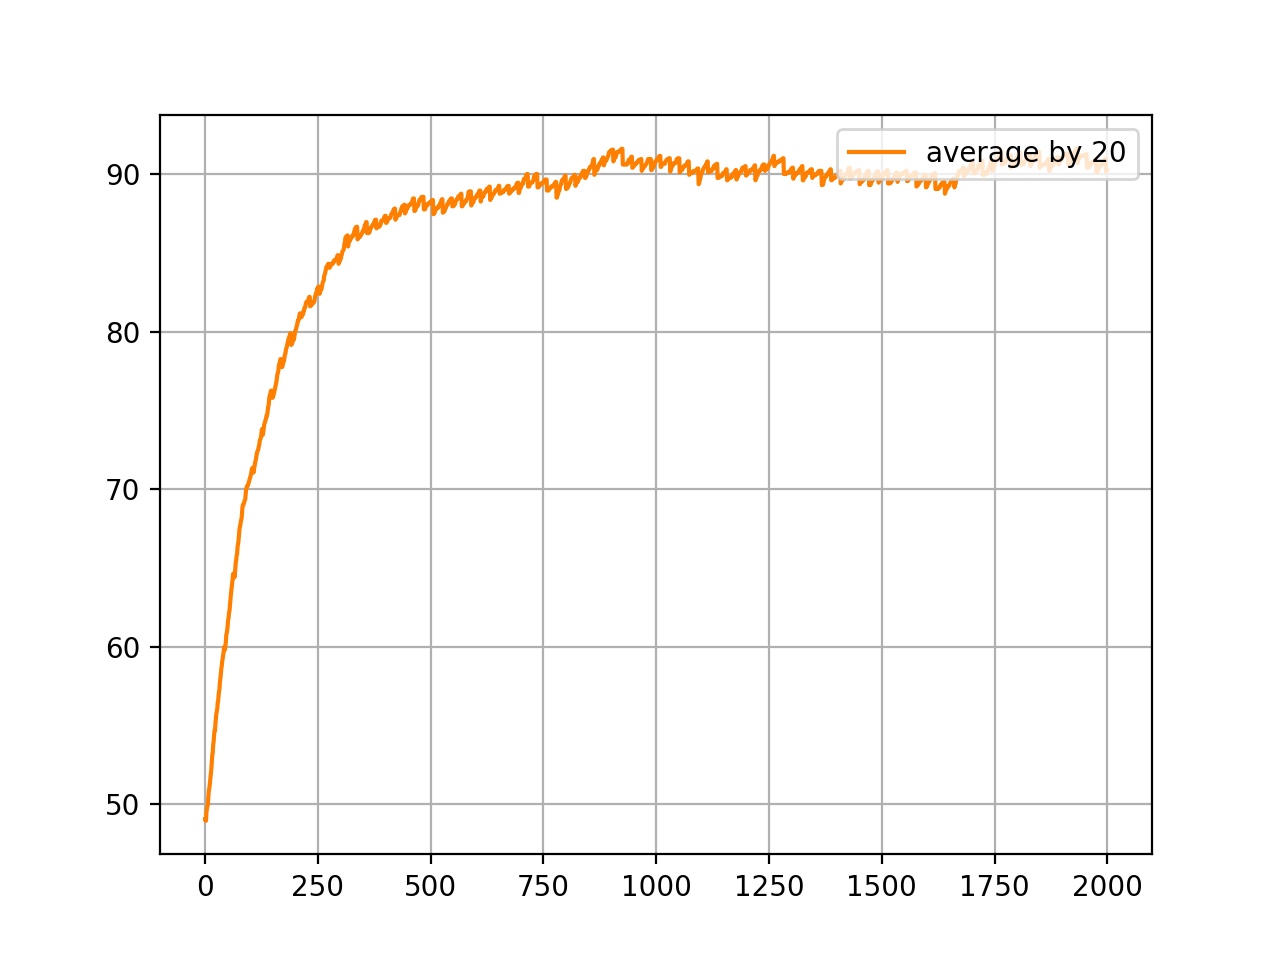
\includegraphics[scale=0.8]{plot_d_averaged_100_1_20_2000.png}
    \end{figure}

    \begin{figure}[H]
        \centering
        \caption{Обнаружение плато с n = 200}
        \label{pic:sublists-metafile}
        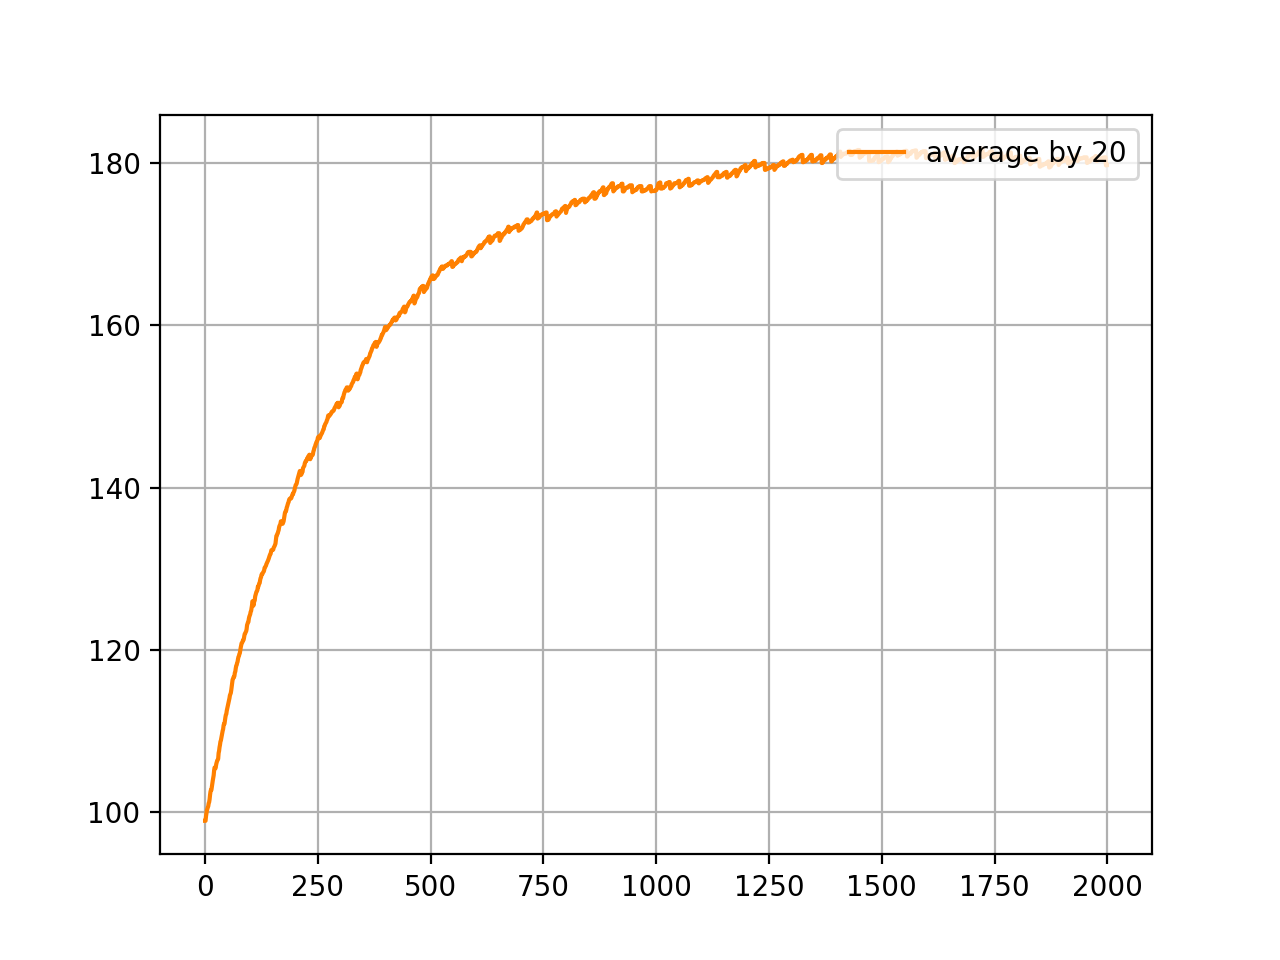
\includegraphics[scale=0.8]{plot_d_averaged_200_1_20_2000.png}
    \end{figure}

    \begin{figure}[H]
        \centering
        \caption{Обнаружение плато с n = 400}
        \label{pic:sublists-metafile}
        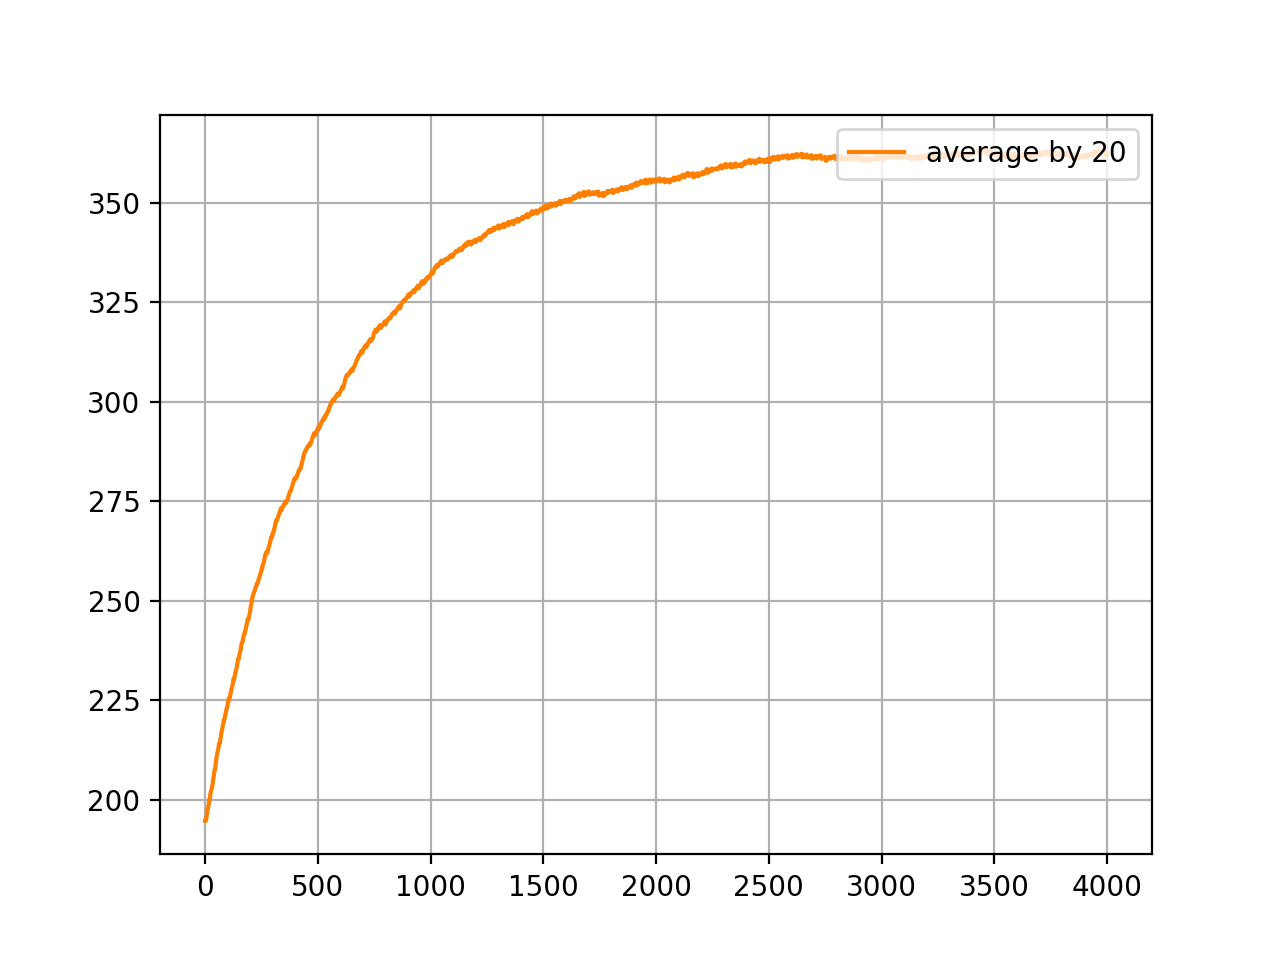
\includegraphics[scale=0.8]{plot_d_averaged_400_1_20_4000.png}
    \end{figure}

    \begin{figure}[H]
        \centering
        \caption{Обнаружение плато с n = 1000}
        \label{pic:sublists-metafile}
        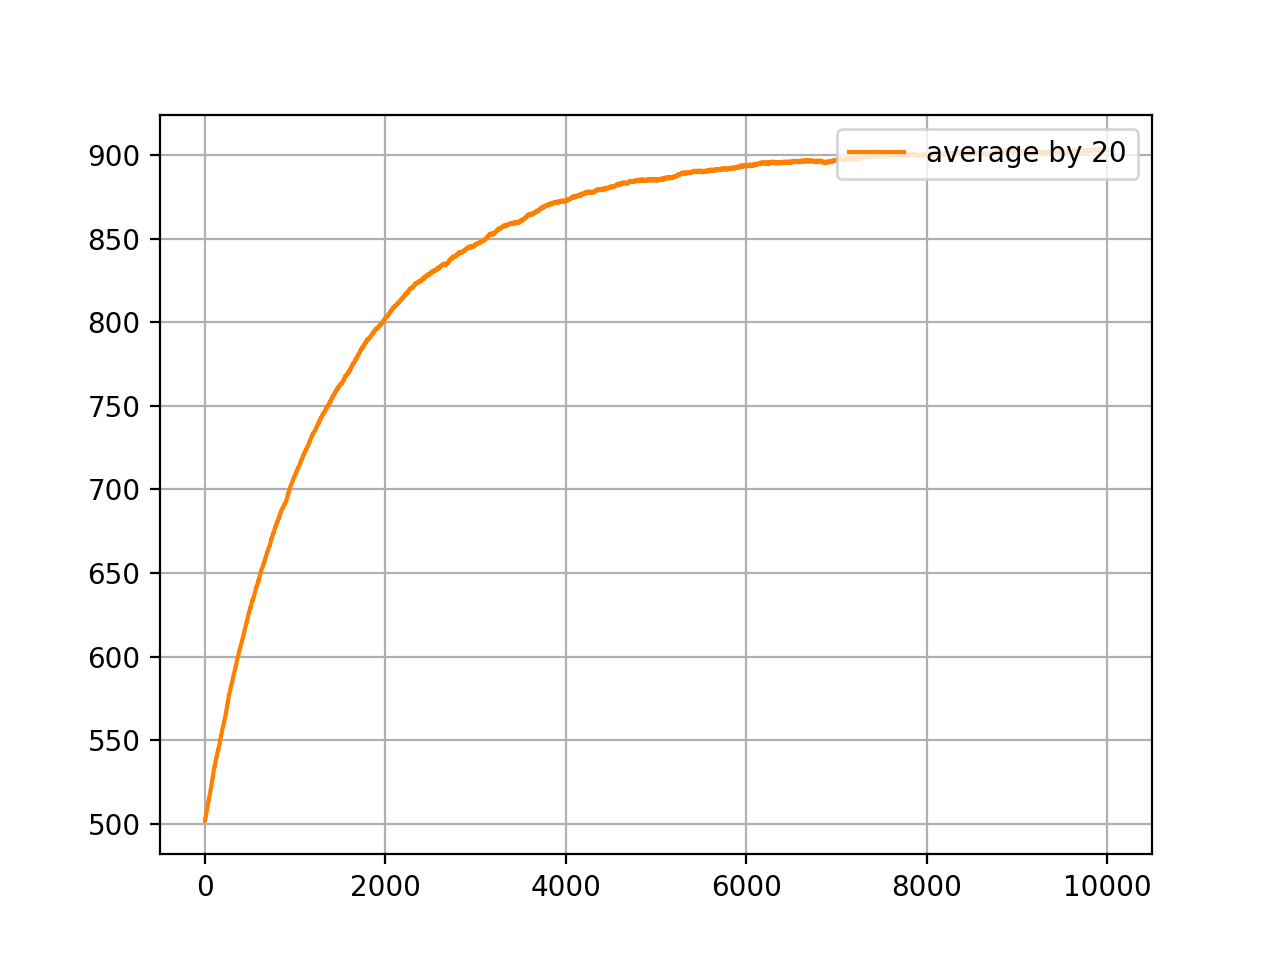
\includegraphics[scale=0.8]{plot_d_averaged_1000_1_20_10000.png}
    \end{figure}


    Для анализа функций $g_{upper}$ и $g_{lower}$ приведены следующие графики:

    \begin{figure}[H]
        \centering
        \caption{Зависимость c и T}
        \label{pic:sublists-metafile}
        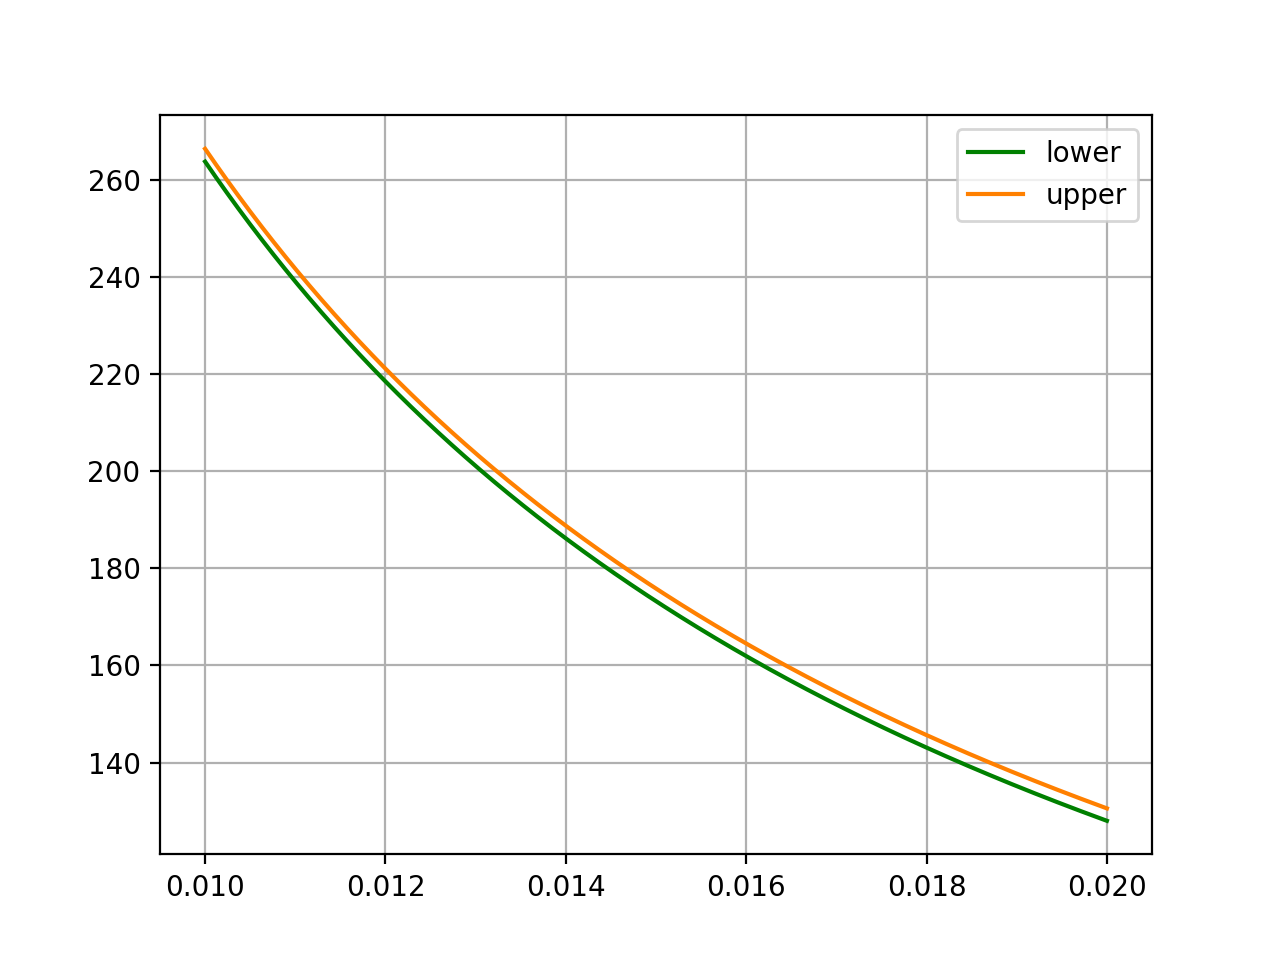
\includegraphics[scale=0.8]{kf_01_02.png}
    \end{figure}
    \begin{figure}[H]
        \centering
        \caption{Зависимость c и T}
        \label{pic:sublists-metafile}
        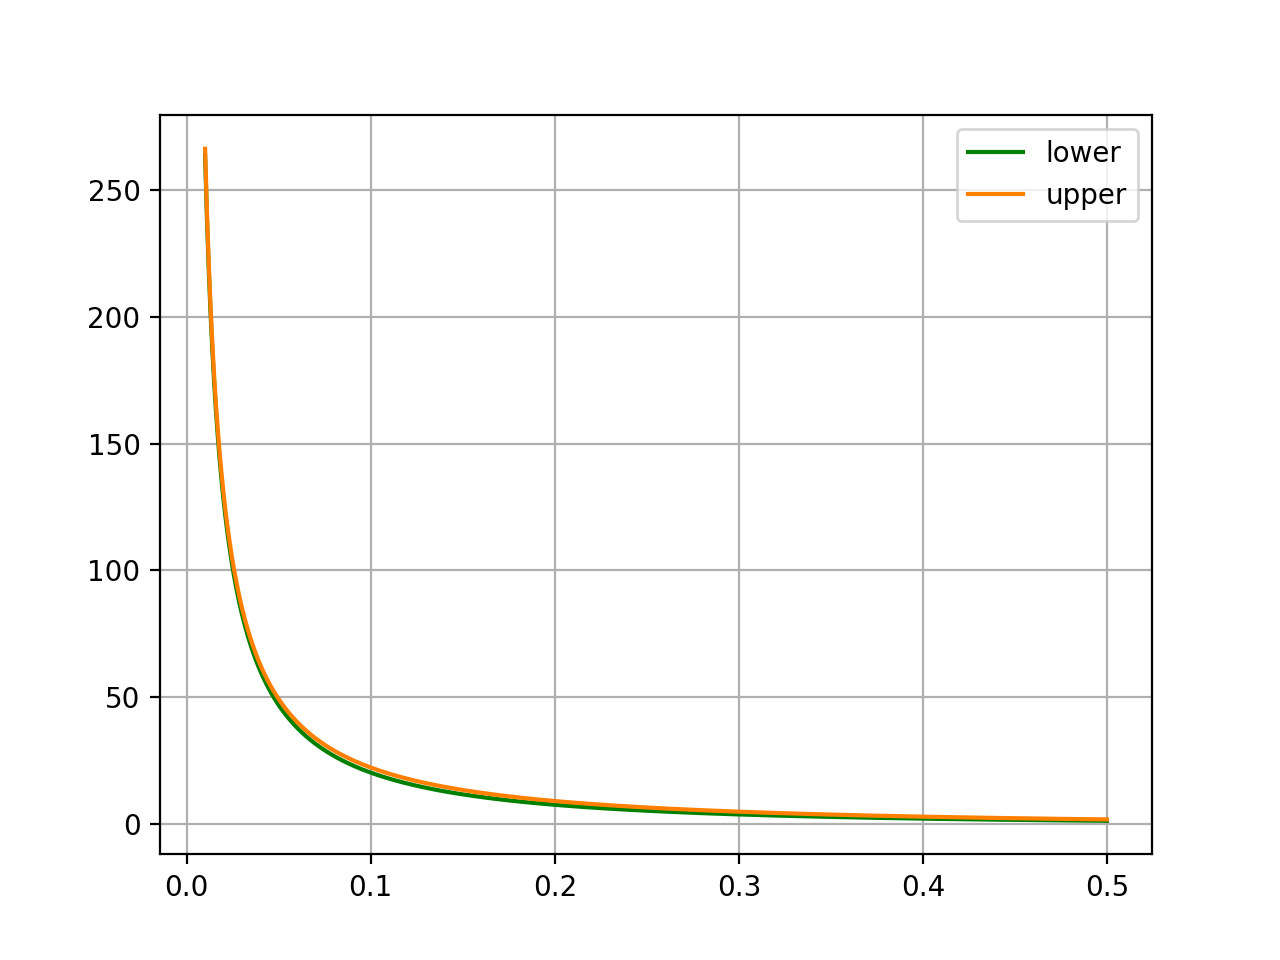
\includegraphics[scale=0.8]{kf_01_5.png}
    \end{figure}
    \begin{figure}[H]
        \centering
        \caption{Зависимость c и T}
        \label{pic:sublists-metafile}
        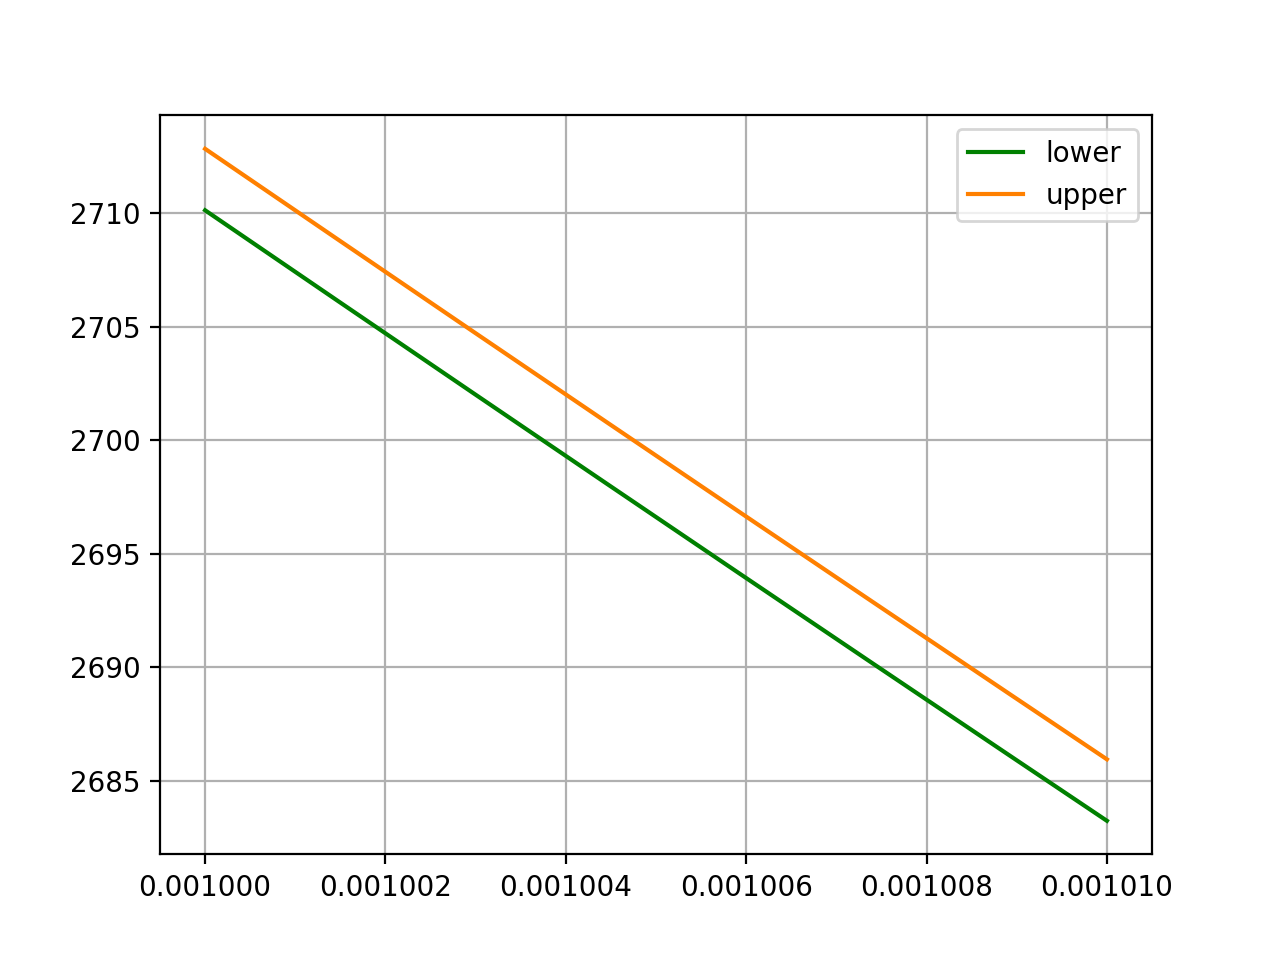
\includegraphics[scale=0.8]{kf_0001_00101.png}
    \end{figure}
    \begin{figure}[H]
        \centering
        \caption{Зависимость c и T}
        \label{pic:sublists-metafile}
        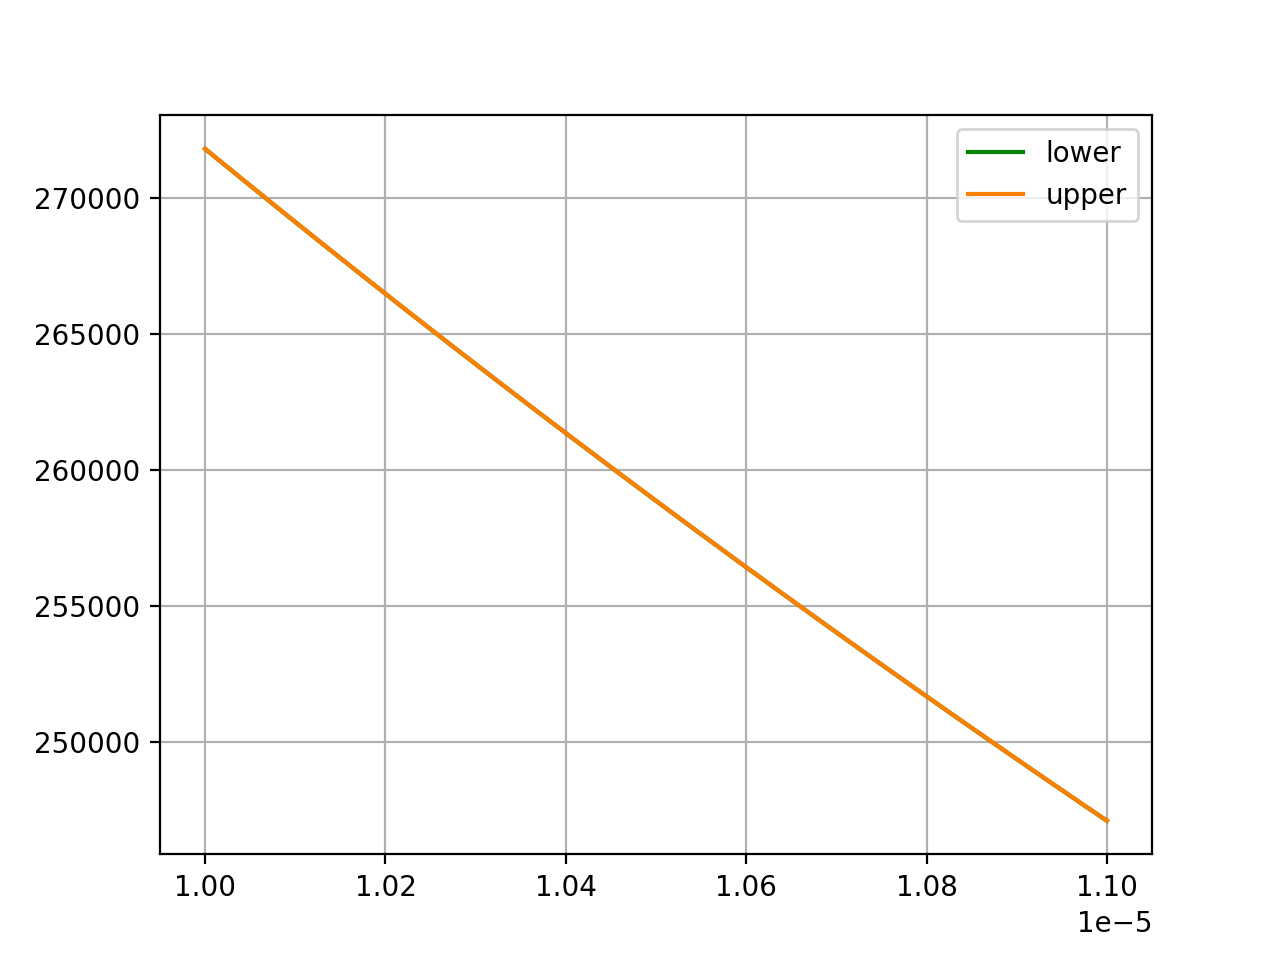
\includegraphics[scale=0.8]{kf_00001_000011.png}
    \end{figure}

    \startconclusionpage
    В результате было обнаружено и доказано несколько теорем, которые помогут в дальнейшим анализировать эволюционные алгоритмы с динамическими изменениями.
    Предсказаны оценки какая точка стабилизация будут находиться для данного T. То есть в каком месте алгоритм будет находиться в независимости от n.
    Выведены пару drift-теорем, которые могут помочь дальнейшим исследованиям динамических оптимизаций, в частности теоремы применены к данной задаче в следствие чего была установлены такие значение T, при которых алгоритм будет находить оптимумы за то же асимптотическое время.
    Так же найдены такие T, в которых алгоритм будет с большой вероятностью в этом оптимуме останавливаться - вероятность его покинуть < какого-то значения или в каких вероятность будет равна o(1)
    Оценки были подтверждены экспериментальными данными.
    \printmainbibliography


\end{document}
